\section{Laboratory work implementation}

\subsection{Tasks and Points}

\begin{itemize}
	\item Basic Level (nota 5 || 6) :
	\begin{itemize}
		\item conecteaza-te la server folosind SSH
		\item compileaza cel putin 2 sample programs din setul HelloWolrdPrograms folosind CLI
		\item executa primul commit folosind VCS
	\end{itemize}
	\item Normal Level (nota 7 || 8):
	\begin{itemize}
		\item initializeaza un nou repositoriu
		\item configureaza-ti VCS
		\item crearea branch-urilor (creeaza cel putin 2 branches)
		\item commit pe ambele branch-uri (cel putin 1 commit per branch)
	\end{itemize}
	\item Advanced Level (nota 9 || 10):
	\begin{itemize}
		\item seteaza un branch to track a remote origin pe care vei putea sa faci push (ex. Github, Bitbucket or custom server)
		\item reseteaza un branch la commit-ul anterior
		\item merge 2 branches
	\item conflict solving between 2 branches
	\end{itemize}
	\end{itemize}

\subsection{Analiza lucrarii de laborator}
GitHub este un serviciu de găzduire web pentru proiecte de dezvoltare a software-ului care utilizează sistemul de control al versiunilor Git. GitHub oferă planuri tarifare pentru depozite private, și conturi gratuite pentru proiecte open source. Site-ul a fost lansat în 2008 de către Tom Preston-Werner, Chris Wanstrath, și PJ Hyett.

\begin{center}

\includegraphics[width=0.7\linewidth]{../../../../../../../../MEGA/midps/GitHub-Logo}
\end{center}
Pentru elaborarea acestui laborator m-am inregistrat pe github,am creat un repozitoriu si am instalat git bash-ul in calculator .
Am reusit sa ma conectez la repozitoriul creat folosind SSH prin git remote add origin email.
Am creeat o cheia ce ma autorizeaza automat prin  ssh-keygen care creeaza o parola autentificarea de la acest device.
\begin{center}

\includegraphics[width=0.7\linewidth]{../../../../../../../../MEGA/midps/addkey}
\end{center}
\begin{center}
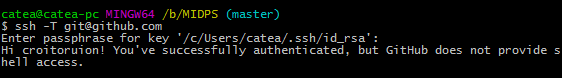
\includegraphics[width=0.7\linewidth]{../../../../../../../../MEGA/midps/ssh_authenticating}
\end{center}

Pentru compilarea si rularea unor programe hello world de exemplu scrise in limbajul java si C++ avem nevoie in primul rand de jdk shi gcc.In setari de la windows introducem calea "path" spre jdk si gcc,pentru compilarea acestor programe in continuare.
Am creat un file java si cpp ,am scris acele hello world programe.
Dupa ce ne-am autentificat in github cu shh-key putem cu ajutorul comenzii javac sa compilam programul jhello iar apoi cu ajutorul comenzii java sa rulam acest program 
\begin{center}
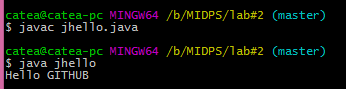
\includegraphics[width=0.7\linewidth]{../../../../../../../../MEGA/midps/JavaCandR}
\end{center}
Pentru a compila si rula un program C++ este comanda g++ "den fisierului" -o "denum file-ului exe"
iar apoi sal rulam cu ajutorul comenzii
./"denumirea fisierului exe"
\begin{center}
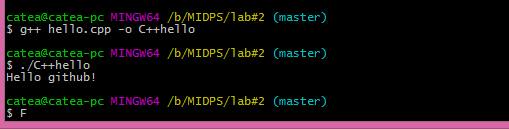
\includegraphics[width=0.7\linewidth]{../../../../../../../../MEGA/midps/C++CandR}
\end{center}

La fiecare push se face si un commit care sistematizeaza orice schimbare pentru o usurare.
Commiturile se fac prin comanda "git commit -m "COMENTARIU" ,iar apoi se face push pentru intrarea in vigoare a schimbarilor noastre
\begin{center}
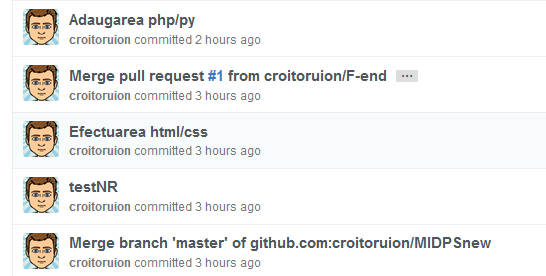
\includegraphics[width=0.7\linewidth]{../../../../../../../../MEGA/midps/commituri}
\end{center}

Am creat un repozitoriu nou MIDPSnew
prin git init,apoi am configurat acest repozitoriu (name/email din github)
\begin{center}
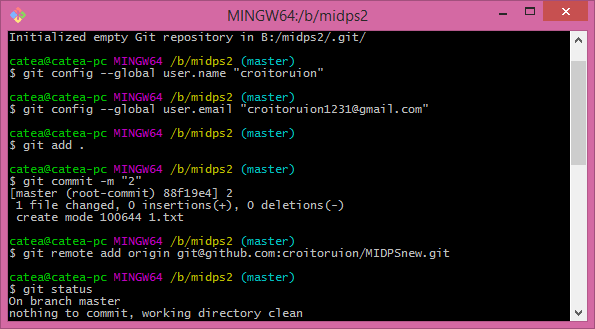
\includegraphics[width=0.7\linewidth]{../../../../../../../../MEGA/midps/newRep}
\end{center}





\begin{center}
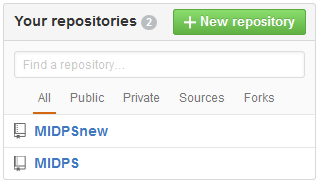
\includegraphics[width=0.7\linewidth]{../../../../../../../../MEGA/midps/rep}
\end{center}

Am creat 2 branch-uri prin ssh cu denumirile F-end si B-end

\begin{center}
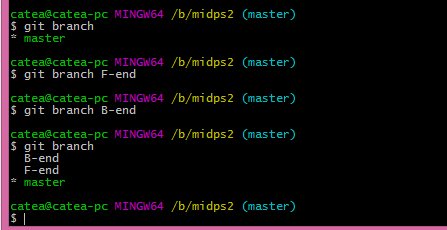
\includegraphics[width=0.7\linewidth]{../../../../../../../../MEGA/midps/2branch}
\end{center}

Am creat 2 fisiere din branch-ul B-end
si le-am adaugat in repozitoriu
\begin{center}
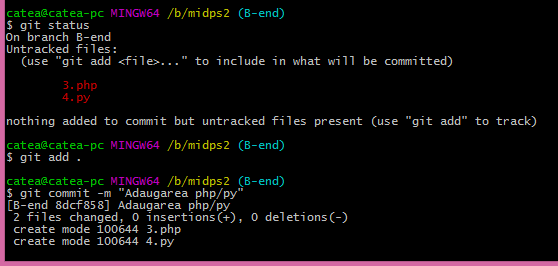
\includegraphics[width=0.7\linewidth]{../../../../../../../../MEGA/midps/Bend}
\end{center}

Observam ca push-ul se face cu ajutorul ssh-key
\begin{center}
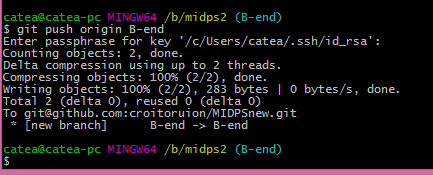
\includegraphics[width=0.7\linewidth]{../../../../../../../../MEGA/midps/Bendpush}
\end{center}

La fel si pentru branch-ul F-end am creat alte 2 fisiere si le-am adaugat in repozitoriu
\begin{center}
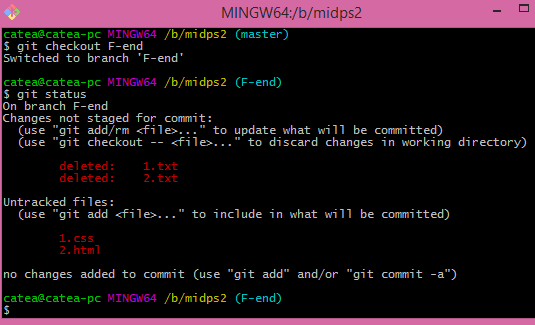
\includegraphics[width=0.7\linewidth]{../../../../../../../../MEGA/midps/Fend}
\end{center}

\begin{center}
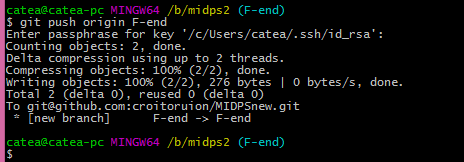
\includegraphics[width=0.7\linewidth]{../../../../../../../../MEGA/midps/Fendpush}
\end{center}


Cand intram pe github in calitate de master observam ca branch-urile noastre creeate au facut push,putem accepta acest push putem sa nu-l acceptam astfel in repozitoriu nu se va schimba nimic.Putem adauga comentarii la acel care a facut acest push/commit
\begin{center}
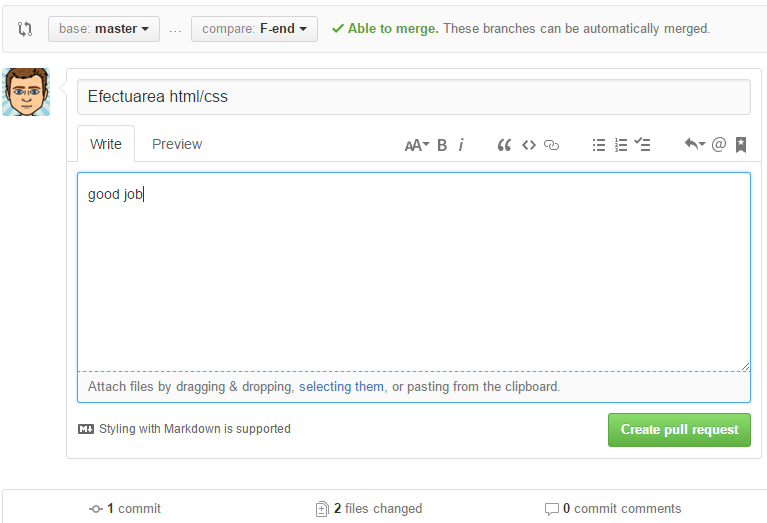
\includegraphics[width=0.7\linewidth]{../../../../../../../../MEGA/midps/acceptareMaster}
\end{center}
Astfel in urma acceptarii ambelor comituri din partea ambelor branch-uri observam ca in repozitoriu a aparut 4 fisiere cate 2 din partea fiecarui branch
\begin{center}
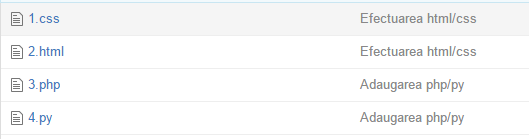
\includegraphics[width=0.7\linewidth]{../../../../../../../../MEGA/midps/branchaccept}
\end{center}


Setam un branch to track remote origin pe care vom putea face push
Am selectat branch-ul B-end
Am facut o schimbare,astfel am facut un commit
\begin{center}
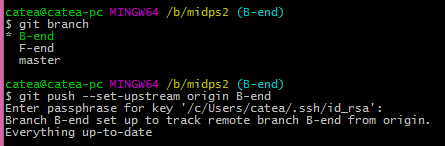
\includegraphics[width=0.7\linewidth]{../../../../../../../../MEGA/midps/trackremote}
\end{center}


Am intrat in log-urile  unde se afla toate commiturile si ne-am reintors la starea anterioara adica la penultimul commit
\begin{center}
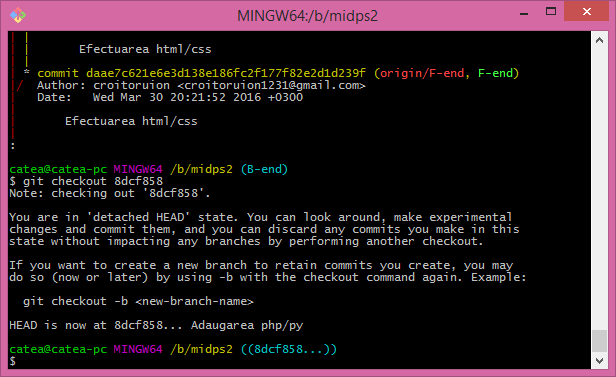
\includegraphics[width=0.7\linewidth]{../../../../../../../../MEGA/midps/backtrack}
\end{center}




Merge 2 branches.
Pentru a face merge la 2 branch-uri utilizam comanda merge.
\begin{center}
\includegraphics[width=0.7\linewidth]{"../../../../../../../../MEGA/midps/Image 004"}
\end{center}

Rezolvarea conflictelor a 2 branch-uri

Am creat 2 fisiere identice dar cu continut diferit in fiecare din branch astfel cand dam merge observam ca apare conflictul
\begin{center}
\includegraphics[width=0.7\linewidth]{"../../../../../../../../MEGA/midps/Image 002"}
\end{center}
Github-ul ne indica si ne ajuta sa rezolvam acest conflict
\begin{center}
\includegraphics[width=0.7\linewidth]{"../../../../../../../../MEGA/midps/Image 003"}
\end{center}
Stergem ce nu ne trebuie si lasam ceea de ce avem nevoie apoi ii dam commit


\clearpage